\documentclass[14pt]{extbook}
\usepackage{multicol, enumerate, enumitem, hyperref, color, soul, setspace, parskip, fancyhdr} %General Packages
\usepackage{amssymb, amsthm, amsmath, bbm, latexsym, units, mathtools} %Math Packages
\everymath{\displaystyle} %All math in Display Style
% Packages with additional options
\usepackage[headsep=0.5cm,headheight=12pt, left=1 in,right= 1 in,top= 1 in,bottom= 1 in]{geometry}
\usepackage[usenames,dvipsnames]{xcolor}
\usepackage{dashrule}  % Package to use the command below to create lines between items
\newcommand{\litem}[1]{\item#1\hspace*{-1cm}\rule{\textwidth}{0.4pt}}
\pagestyle{fancy}
\lhead{Progress Quiz 4}
\chead{}
\rhead{Version A}
\lfoot{6286-1986}
\cfoot{}
\rfoot{Fall 2020}
\begin{document}

\begin{enumerate}
\litem{
Factor the quadratic below. Then, choose the intervals that contain the constants in the form $(ax+b)(cx+d); b \leq d.$\[ 54x^{2} +57 x + 10 \]\begin{enumerate}[label=\Alph*.]
\item \( a \in [0.4, 3.8], \hspace*{5mm} b \in [11, 14], \hspace*{5mm} c \in [-0.86, 1.37], \text{ and } \hspace*{5mm} d \in [44, 47] \)
\item \( a \in [6.4, 12.8], \hspace*{5mm} b \in [0, 3], \hspace*{5mm} c \in [5.93, 7.07], \text{ and } \hspace*{5mm} d \in [3, 6] \)
\item \( a \in [3.4, 5.1], \hspace*{5mm} b \in [0, 3], \hspace*{5mm} c \in [10.7, 12.92], \text{ and } \hspace*{5mm} d \in [3, 6] \)
\item \( a \in [24.8, 27.6], \hspace*{5mm} b \in [0, 3], \hspace*{5mm} c \in [1.41, 2.32], \text{ and } \hspace*{5mm} d \in [3, 6] \)
\item \( \text{None of the above.} \)

\end{enumerate} }
\litem{
Solve the quadratic equation below. Then, choose the intervals that the solutions belong to, with $x_1 \leq x_2$ (if they exist).\[ 17x^{2} +12 x -9 = 0 \]\begin{enumerate}[label=\Alph*.]
\item \( x_1 \in [-28.28, -27.48] \text{ and } x_2 \in [26.99, 27.36] \)
\item \( x_1 \in [-1.54, -0.96] \text{ and } x_2 \in [-0.63, 1.02] \)
\item \( x_1 \in [-1.03, -0.43] \text{ and } x_2 \in [0.59, 1.5] \)
\item \( x_1 \in [-19.92, -19.53] \text{ and } x_2 \in [7.43, 8.2] \)
\item \( \text{There are no Real solutions.} \)

\end{enumerate} }
\litem{
Write the equation of the graph presented below in the form $f(x)=ax^2+bx+c$, assuming  $a=1$ or $a=-1$. Then, choose the intervals that $a, b,$ and $c$ belong to.
\begin{center}
    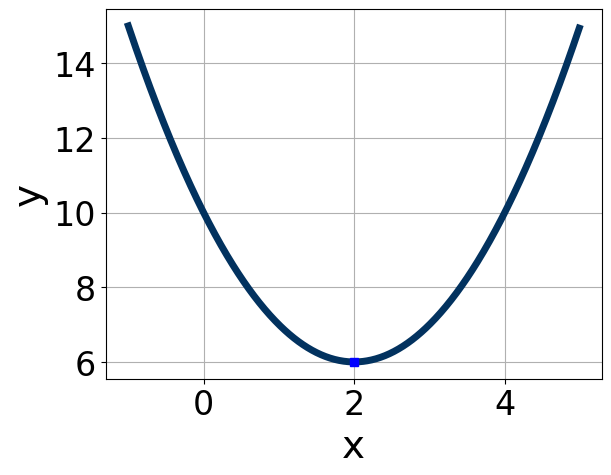
\includegraphics[width=0.5\textwidth]{../Figures/quadraticGraphToEquationA.png}
\end{center}
\begin{enumerate}[label=\Alph*.]
\item \( a \in [-0.3, 1.9], \hspace*{5mm} b \in [8, 9], \text{ and } \hspace*{5mm} c \in [8, 13] \)
\item \( a \in [-1.6, 0.3], \hspace*{5mm} b \in [-10, -6], \text{ and } \hspace*{5mm} c \in [-22, -21] \)
\item \( a \in [-0.3, 1.9], \hspace*{5mm} b \in [-10, -6], \text{ and } \hspace*{5mm} c \in [8, 13] \)
\item \( a \in [-0.3, 1.9], \hspace*{5mm} b \in [8, 9], \text{ and } \hspace*{5mm} c \in [20, 25] \)
\item \( a \in [-1.6, 0.3], \hspace*{5mm} b \in [8, 9], \text{ and } \hspace*{5mm} c \in [-22, -21] \)

\end{enumerate} }
\litem{
Graph the equation below.\[ f(x) = (x+2)^2 + 14 \]\begin{enumerate}[label=\Alph*.]
\begin{multicols}{2}\item 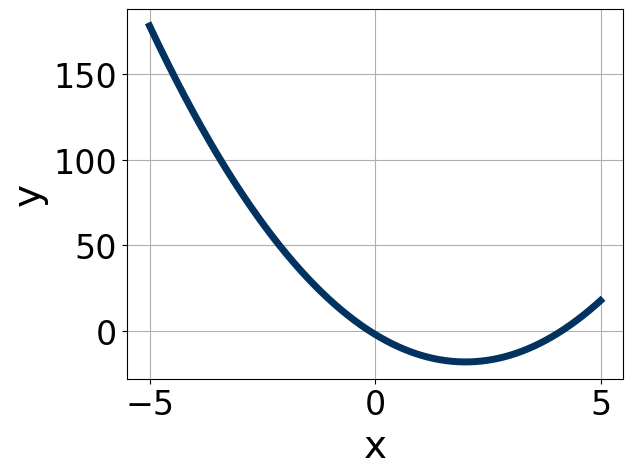
\includegraphics[width = 0.3\textwidth]{../Figures/quadraticEquationToGraphAA.png}\item 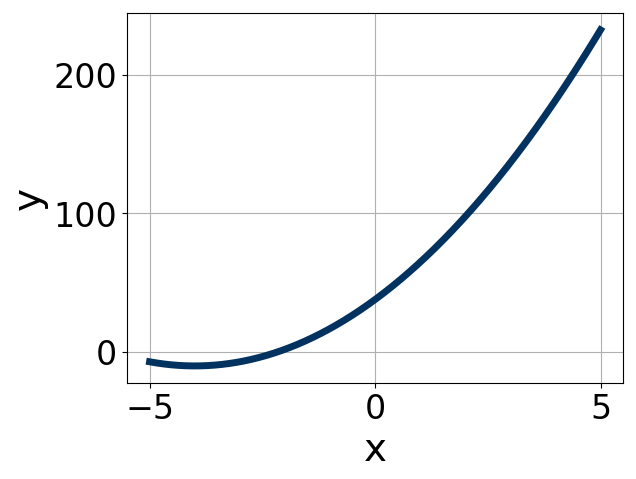
\includegraphics[width = 0.3\textwidth]{../Figures/quadraticEquationToGraphBA.png}\item 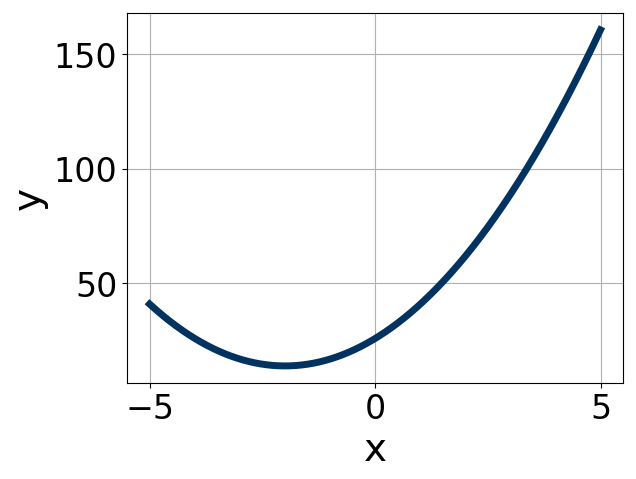
\includegraphics[width = 0.3\textwidth]{../Figures/quadraticEquationToGraphCA.png}\item 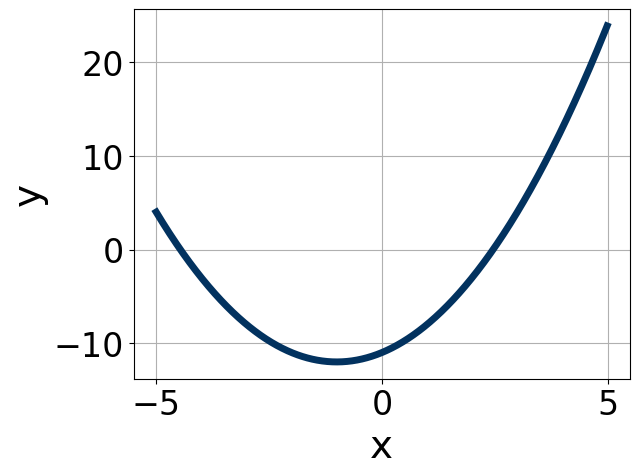
\includegraphics[width = 0.3\textwidth]{../Figures/quadraticEquationToGraphDA.png}\end{multicols}\item None of the above.
\end{enumerate} }
\litem{
Write the equation of the graph presented below in the form $f(x)=ax^2+bx+c$, assuming  $a=1$ or $a=-1$. Then, choose the intervals that $a, b,$ and $c$ belong to.
\begin{center}
    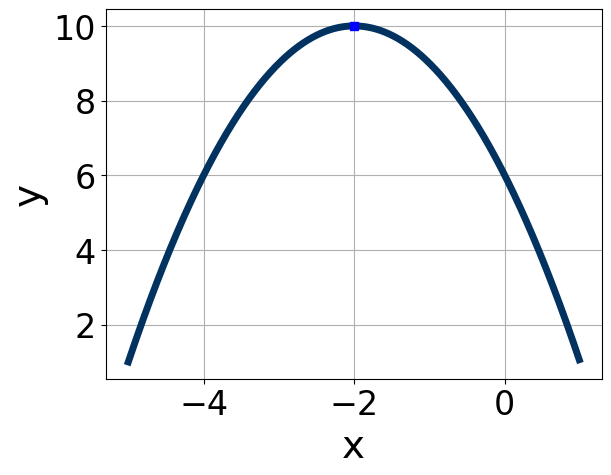
\includegraphics[width=0.5\textwidth]{../Figures/quadraticGraphToEquationCopyA.png}
\end{center}
\begin{enumerate}[label=\Alph*.]
\item \( a \in [0, 1.8], \hspace*{5mm} b \in [1, 7], \text{ and } \hspace*{5mm} c \in [13, 15] \)
\item \( a \in [-1.1, 0.7], \hspace*{5mm} b \in [-5, 2], \text{ and } \hspace*{5mm} c \in [-15, -12] \)
\item \( a \in [-1.1, 0.7], \hspace*{5mm} b \in [1, 7], \text{ and } \hspace*{5mm} c \in [6, 7] \)
\item \( a \in [0, 1.8], \hspace*{5mm} b \in [-5, 2], \text{ and } \hspace*{5mm} c \in [13, 15] \)
\item \( a \in [-1.1, 0.7], \hspace*{5mm} b \in [-5, 2], \text{ and } \hspace*{5mm} c \in [6, 7] \)

\end{enumerate} }
\litem{
Graph the equation below.\[ f(x) = -(x-2)^2 + 15 \]\begin{enumerate}[label=\Alph*.]
\begin{multicols}{2}\item 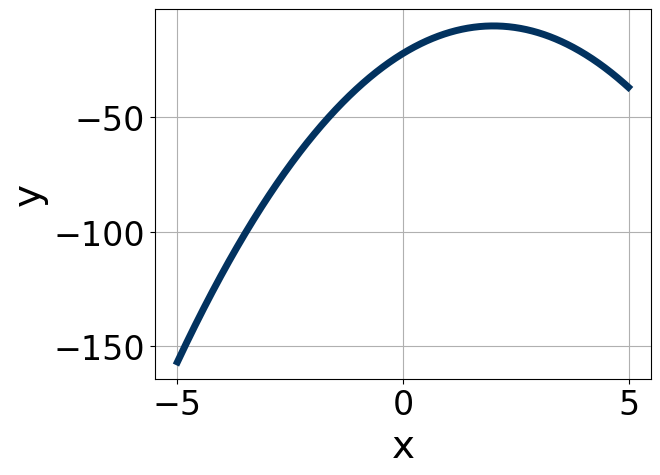
\includegraphics[width = 0.3\textwidth]{../Figures/quadraticEquationToGraphCopyAA.png}\item 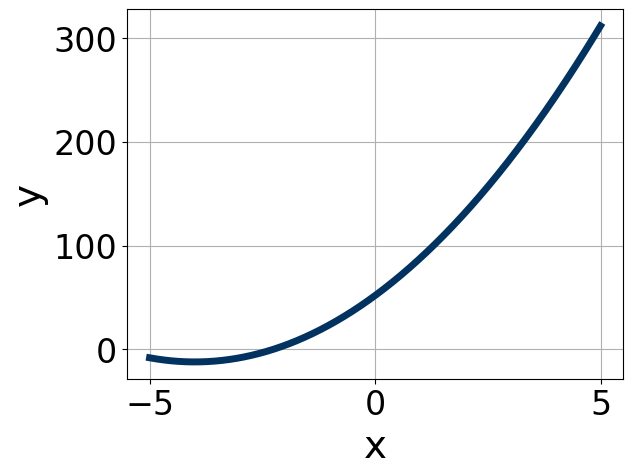
\includegraphics[width = 0.3\textwidth]{../Figures/quadraticEquationToGraphCopyBA.png}\item 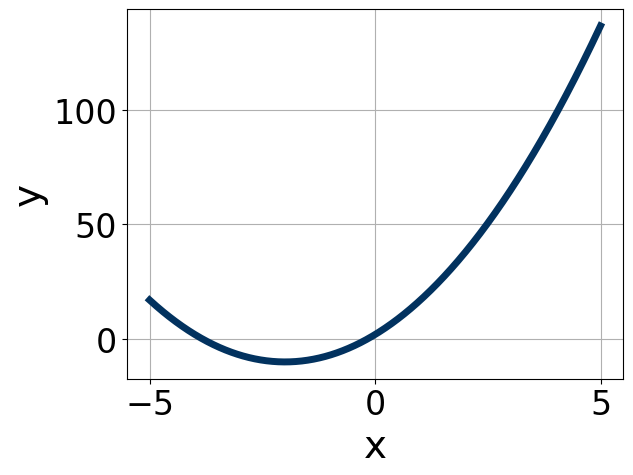
\includegraphics[width = 0.3\textwidth]{../Figures/quadraticEquationToGraphCopyCA.png}\item 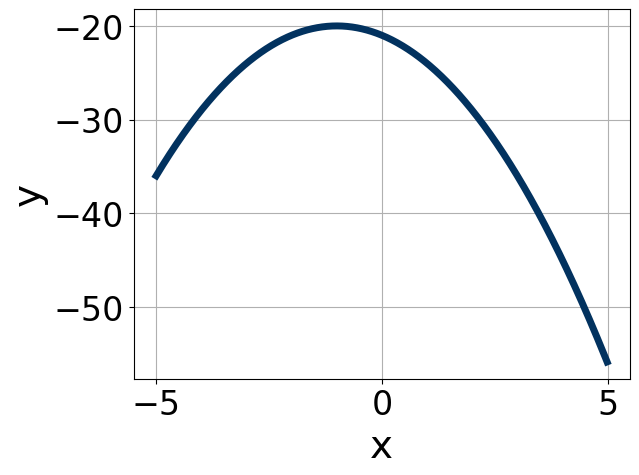
\includegraphics[width = 0.3\textwidth]{../Figures/quadraticEquationToGraphCopyDA.png}\end{multicols}\item None of the above.
\end{enumerate} }
\litem{
Factor the quadratic below. Then, choose the intervals that contain the constants in the form $(ax+b)(cx+d); b \leq d.$\[ 16x^{2} -32 x + 15 \]\begin{enumerate}[label=\Alph*.]
\item \( a \in [1.76, 2.51], \hspace*{5mm} b \in [-10, -2], \hspace*{5mm} c \in [6.8, 9.17], \text{ and } \hspace*{5mm} d \in [-3, 0] \)
\item \( a \in [6.86, 8.53], \hspace*{5mm} b \in [-10, -2], \hspace*{5mm} c \in [1.41, 2.13], \text{ and } \hspace*{5mm} d \in [-3, 0] \)
\item \( a \in [2.39, 4.25], \hspace*{5mm} b \in [-10, -2], \hspace*{5mm} c \in [2.38, 4.86], \text{ and } \hspace*{5mm} d \in [-3, 0] \)
\item \( a \in [0.55, 1.39], \hspace*{5mm} b \in [-20, -16], \hspace*{5mm} c \in [0.19, 1.2], \text{ and } \hspace*{5mm} d \in [-12, -8] \)
\item \( \text{None of the above.} \)

\end{enumerate} }
\litem{
Solve the quadratic equation below. Then, choose the intervals that the solutions $x_1$ and $x_2$ belong to, with $x_1 \leq x_2$.\[ 20x^{2} +21 x -54 = 0 \]\begin{enumerate}[label=\Alph*.]
\item \( x_1 \in [-4.6, -2.77] \text{ and } x_2 \in [0.47, 0.91] \)
\item \( x_1 \in [-10.17, -8.65] \text{ and } x_2 \in [0.21, 0.51] \)
\item \( x_1 \in [-0.91, -0.74] \text{ and } x_2 \in [3.41, 3.82] \)
\item \( x_1 \in [-2.93, -1.14] \text{ and } x_2 \in [0.7, 1.57] \)
\item \( x_1 \in [-46.76, -44.28] \text{ and } x_2 \in [23.04, 24.03] \)

\end{enumerate} }
\litem{
Solve the quadratic equation below. Then, choose the intervals that the solutions belong to, with $x_1 \leq x_2$ (if they exist).\[ 15x^{2} -15 x -9 = 0 \]\begin{enumerate}[label=\Alph*.]
\item \( x_1 \in [-29, -26.9] \text{ and } x_2 \in [27.94, 28.59] \)
\item \( x_1 \in [-1.4, 1] \text{ and } x_2 \in [1.06, 1.77] \)
\item \( x_1 \in [-7.6, -6.1] \text{ and } x_2 \in [20.45, 22.18] \)
\item \( x_1 \in [-2.7, -0.9] \text{ and } x_2 \in [0.38, 0.63] \)
\item \( \text{There are no Real solutions.} \)

\end{enumerate} }
\litem{
Solve the quadratic equation below. Then, choose the intervals that the solutions $x_1$ and $x_2$ belong to, with $x_1 \leq x_2$.\[ 25x^{2} +60 x + 36 = 0 \]\begin{enumerate}[label=\Alph*.]
\item \( x_1 \in [-2.98, -1.29] \text{ and } x_2 \in [-0.69, -0.42] \)
\item \( x_1 \in [-2.13, -0.94] \text{ and } x_2 \in [-1.28, -0.97] \)
\item \( x_1 \in [-30.73, -28.36] \text{ and } x_2 \in [-30.12, -29.88] \)
\item \( x_1 \in [-7.75, -4.14] \text{ and } x_2 \in [-0.27, -0.11] \)
\item \( x_1 \in [-4.05, -3.34] \text{ and } x_2 \in [-0.45, -0.39] \)

\end{enumerate} }
\end{enumerate}

\end{document}